\chapter{Einleitung}

\section{Hintergrund \& Motivation}

In Zeiten der Globalisierung ist es für Großkonzerne von großer Bedeutung, Prozesse zu vereinfachen, um Ressourcen und Kapazitäten einzusparen. Vor allem in der \ac{IT} ist Optimierungspotential vorhanden, da hier viele Prozesse und Arbeitsvorgänge immer noch nicht vereinheitlicht sind.
Nicht standardisierte Prozesse sowie individuelle Software führen zu erhöhtem Aufwand für IT-Personal, als auch für die einzelnen Gesellschaften.

\ac{ABB} ist ein global f\"{u}hrender Hersteller und Serviceanbieter in der Energie- und Automatisierungstechnik mit Hauptsitz in Z\"{u}rich.
Der internationale Konzern entstand 1988 aus der Fusion des schwedischen Unternehmens \ac{ASEA} und der schweizerischen Firma \ac{BBC}. ABB besch\"{a}ftigt zurzeit \"{u}ber 132.000 Mitarbeiter in 100 L\"{a}ndern. Im Jahr 2016 wurde ein weltweiter Umsatz von 33,8 Mrd. USD und ein Nettogewinn von 2,1 Mrd USD erwirtschaftet.\footnote{Vgl. \cite{ABB.2017}} 




\begin{figure}[ht]
	\centering
	\makebox[\textwidth][c]{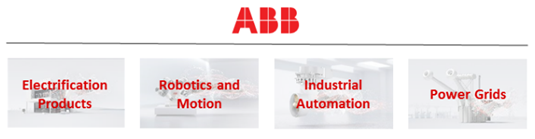
\includegraphics[width=1\textwidth]{img/ABB-Div.png}}%
	
	\caption{Divisionen von \acs{ABB}}
	\label{fig1}
	
\end{figure}

Das Produktportfolio von \ac{ABB} gliedert sich in vier Divisionen auf: Division Electrification, Robotics and Motion, Industrial Automation und Power Grids. Diese Aufteilung ist auch in Abbildung \ref{fig1} zu sehen.

Der Bereich \ac{DE-IS} fungiert als Koordinator der IT-Kernfunktionen der \ac{ABB} Deutschland, sowie teilweise für Zentraleuropa. In enger Zusammenarbeit mit den operativen Einheiten werden unter anderem folgende Aufgaben wahrgenommen:

\begin{itemize}
	\item Vertretung der \ac{ABB} in Deutschland gegenüber diversen Serviceprovidern wie beispielsweise der \ac{IBM}
	\item Unterstützung des operativen Geschäfts mit Hilfe von informationstechnischen und applikativen  Lösungen, sowie der Betreuung dieser.
	\item Verwaltung laufender IS-Betriebsprozesse in Abstimmung mit den IS-Verant-wortlichen vor Ort
	\item Administration und Erweiterung des \ac{ERP}-Systems der \ac{ABB} AG
\end{itemize}


 Trotz der überregionalen Verantwortung gibt es innerhalb der verschiedenen Gesellschaften des \ac{ABB}-Konzerns unterschiedliche Arbeitsweisen, welche noch nicht standardisiert sind. Dies hat zur Folge, dass Prozesse unterschiedlich lang andauern und unterschiedlich hohe Kosten verursachen. Auch werden parallel dieselben Aufgabenstellungen in verschiedenen Abteilungen auf die gleiche Art gelöst und könnten somit von einem zentralisierten Prozess sehr profitieren. Beispielsweise werden beim Versand von Waren innerhalb der \ac{EU} Lieferantenerklärungen ausgestellt, um den Zollbestimmungen gerecht zu werden. Bisher werden diese Dokumente individuell für die jeweilige ABB-Gesellschaft erstellt, sodass bei Änderungen der Zollbestimmungen oder anderen Anpassungen mehrere Dokumente bearbeitet werden müssen.
 
 Hintergrund dieser Arbeit ist eine technische Zusammenführung selbiger Dokumente in eine homogene \acf{LLE} für alle Gesellschaften. Hiermit wird der Veränderungsprozess verkürzt und vereinfacht, sowie die Ausgabe von \ac{ABB}-Dokumenten vereinheitlicht. Mit Hilfe der Adobe Interactive Forms im SAP ERP-System sollen diese Anforderungen umgesetzt werden.

\section{Zielsetzung}

Ziel dieser Arbeit ist das Harmonisieren eines aktuell gesellschaftsspezifischen Formulars in Form eines Adobe \ac{PDF}. Zwar sollen die verschiedenen Dokumente technisch zu einem zusammengefasst werden, jedoch soll es weiterhin möglich sein, dynamisch Inhalte nur für bestimmte Bereiche darzustellen. Beispielsweise besteht die Anforderung, unterschiedliche Firmenlogos an verschiedenen Positionen anzuzeigen. Obendrein gilt es das neue Formular in einer Weise zu erstellen, welche weitere Anpassungen vereinfacht und eine technische Übersichtlichkeit bietet.
Hierzu müssen sich überschneidende Elemente zusammengeführt werden, sowie die Vorgehensweise in der Erstellung des neuen Dokumentes deutlich und nachvollziehbar durchgeführt werden.

\section{Vorgehen}


Zunächst werden in Kapitel \ref{ch:Grundlagen} nötige Grundlagen für das Verständnis der Arbeit erläutert. Auf Basis der Ist-Analyse in Kapitel \ref{ch:Ist-Analyse} werden im nächsten Kapitel unternehmensspezifische Anforderungen analysiert und ausgearbeitet. Danach folgen der Entwurf, sowie dessen technische Umsetzung, welche auf der Anforderungsanalyse aufbaut. Hierbei werden verschiedene Lösungsansätze erläutert und bewertet. Abschließend werden die Erkenntnisse und Ergebnisse in einem Fazit wiedergespiegelt, sowie ein Ausblick auf die Zukunft gegeben.